\section{Wojciech Matuszyński}

\hfill

\subsection{Krótki tekst}

Kierunek Cyberbezpieczeństwo...

\hfill

Kierunek cyberbezpieczeństwo dostarczy absolwentów, którzy będą niezbędnymi ogniwami pozwalającymi realizować kierunki rozwoju gospodarki Polski zapisane w strategicznych dokumentach takich jak choćby w Strategii na rzecz Odpowiedzialnego Rozwoju.
\par
W ten sposób kierunek cyberbezpieczeństwo wpisuje się nie tylko w misję AGH, wydziału IEiT, ale i szerzej w strategiczne kierunki rozwoju Polski, a nawet Europy.

\subsection{Zdjęcie}

\begin{figure}[h!]
  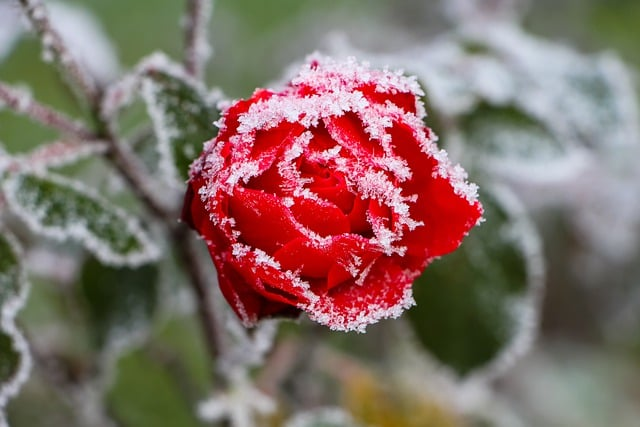
\includegraphics[width=10cm]{pictures/rose-gc0a189534_640.jpg}
  \centering
  \caption{Ośnieżona róża}
  \label{fig:roza}
\end{figure}

\subsection{Wyrażenie matematyczne}

\hfill
\hfill

f(x)=\left\{ \begin{array}{lr} x+1 & dla \ x\in(-\infty;0) \\ x-1 & dla \ x\in\langle0;+\infty) \end{array}\right

\subsection{Tabela}

\begin{table}[]
\begin{tabular}{|l|l|l|l|l|}
\hline
C & Y & B & E & R  \\ \hline
B & E & Z & P & I  \\ \hline
E & C & Z & E & Ń  \\ \hline
S & T & W & O & :) \\ \hline
\end{tabular}
\end{table}

\subsection{Listy}


Lista numerowana:
\begin{enumerate}
  \item Jeden
  \item Dwa
  \item Tri
\end{enumerate}

Lista nienumerowana:
\begin{itemize}
  \item pierwsza
  \item druga
  \item trzecia
\end{itemize}